% ------------------------------------------------------------
\section{Ablation Study}
\label{sec:ablations}
% ------------------------------------------------------------

We analyse the pipeline along four dimensions, namely its architecture, the quality of the descriptions Stage~2 produces, the content those descriptions should carry, and its failure profile against the strongest baseline. Each ablation isolates a single design decision or a single foundation model, locating where the pipeline gains accuracy and where it remains limited on a task none of its constituent models was built to solve. 

\begin{table}[h]
  \centering
  \setlength{\tabcolsep}{4pt}
  \caption{Contribution of each pipeline component on 10\% of the validation takes, \textit{Ego2Exo} direction.}
  \label{tab:abl-summary}
  \begin{tabular}{lrrr}
  \toprule
  Exp. & IoU$\uparrow$ & $t$/frame\,(s)$\downarrow$ & Total$\downarrow$ \\
  \midrule
  Baseline & 0.1059 & 1.32 & 3h\,50m \\
  Baseline Oracle & 0.1703 & 0.12 & 21m\,20s \\
  \midrule
  (A) Best Single Frame & 0.1684 & 0.13 & 22m\,53s \\
  (B) SAM3 Agent Loop & 0.3554 & 21.30 & 59h\,15m \\
  (C) Propagation & 0.3769 & 0.82 & 2h\,23m \\
  (D) G-DINO & \textbf{0.3751} & 0.90 & 2h\,37m \\
  \midrule
  \shortstack[l]{D \% change w.r.t.\\ Baseline $\tfrac{x-y}{y}$}
    & \textcolor[rgb]{0,0.55,0}{$+254.2\%$}
    & \textcolor[rgb]{0,0.55,0}{$-31.8\%$}
    & \textcolor[rgb]{0,0.55,0}{$-31.7\%$} \\
  \bottomrule
  \end{tabular}
\end{table}

\paragraph{Pipeline architecture.}
\Cref{tab:abl-summary} traces the contribution of each component on the \textit{Ego2Exo} direction by adding the stages of \cref{sec:method-overview} one at a time. Unless otherwise specified, the following experiments are run on 10\% of the validation set. The baseline queries the VLM independently on every source frame, runs SAM~3 once per destination frame, and reaches an IoU of 0.106 at 1.32\,s per frame. Replacing the generated description with the ground truth object name (Baseline Oracle) lifts IoU to 0.170, which already isolates description quality as a primary bottleneck before any architectural change is made.

Generating a description on every source frame is redundant, because the object's appearance barely changes across a take. Experiment~A selects a single salient source frame through the composite visibility score of \cref{eq:frame-score} and recovers nearly all of the oracle gain (IoU 0.168 at 0.13\,s per frame) without any privileged information. This confirms the premise of Stage~1 (\cref{subsec:Stage1}), that a clearer source frame yields a better description than the average annotated one. We adopt the composite score rather than a simpler rule because further experiments isolate where its value comes from. Selecting the single frame at random loses 4.7 percentage points of IoU against it, which shows that the choice of frame matters, whereas richer engineered colour prompts and several frames of temporal context both underperform, since their verbose phrasing is incompatible with the short noun phrases the SAM~3 encoder was trained on. A clearer source frame helps; a more elaborate description does not.

Experiment~B applies the full SAM~3 agent loop on every destination frame and reaches IoU 0.355, but the repeated tool calls raise latency to 21.30\,s per frame, raising total run time to 59 hours, which is impractical at scale. Experiment~C addresses the cost with propagation, matching that accuracy (IoU 0.377) at 0.82\,s per frame, roughly 25 times faster. Together, B and C establish propagation as the efficient route to high accuracy on each frame and reinforce the principle behind the split of \cref{sec:task-formulation}, that transfer across views need only succeed on a few destination frames for the tracker to complete the rest.

To address the asymmetry in mask quality between the two views, Experiment~D adds the anchor selection signal of Stage~3. Grounding DINO yields IoU 0.375 at 0.90\,s per frame, a relative improvement of 254.2\% over the baseline, although the gain over propagation alone falls within the noise of the small ablation subset. Selecting anchors by language thus matches propagation on this subset while keeping the bridge across views entirely linguistic, which is why we adopt it as the anchor signal of the full pipeline. A geometric alternative based on dense matching is unattractive here, since such correspondences collapse under the viewpoint gap between the egocentric and exocentric views (\cref{subsec:matching}).

\paragraph{Anchor selection and count.}
Two choices govern Stage~3, namely where the anchors come from and how many we keep. The two views are roughly synchronised in time, so the simplest rule would transfer the mask at the destination frame that shares the chosen source frame's index. However, synchronisation in time does not imply alignment in appearance, since at the same instant the target can be occluded, tiny, or out of frame in the destination view, so the best source frame is rarely the best destination frame. \Cref{fig:anchor-selection} confirms this, since the composite scores of paired source and destination frames are almost uncorrelated, with a Spearman correlation of 0.14 across frames and a distribution within each object centred on zero, so a frame that scores well in one view carries no guarantee of scoring well in the other. Stage~3 therefore selects anchors independently in the destination view by grounding confidence rather than reusing the source index. \Cref{tab:abl-anchors} supports this separation, as drawing anchors at random costs 4.4 percentage points of IoU in \textit{Ego2Exo} and 2.6 in \textit{Exo2Ego} against selection ranked by confidence at the same count.

\begin{figure}
    \centering
    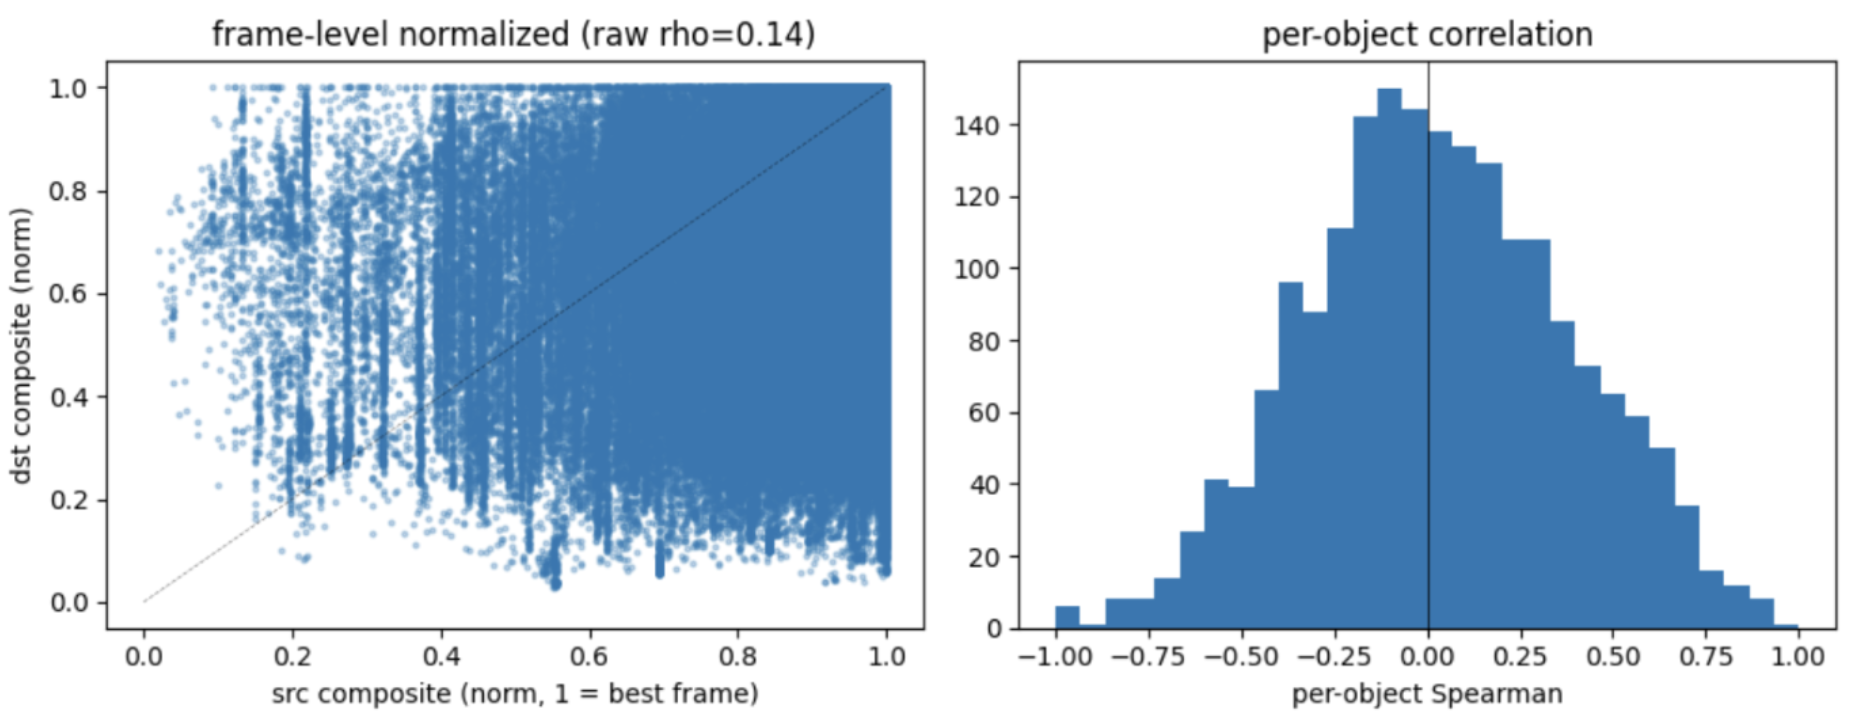
\includegraphics[width=\linewidth]{imgs/ch4/anchor-selection.png}
    \caption{Composite visibility scores do not transfer across views. On the left, the normalised composite score of each source frame plotted against the score of its paired destination frame, with a Spearman correlation of 0.14. On the right, the distribution of that correlation computed within each object, centred on zero. A frame that scores well in one view is therefore rarely the best frame in the other.}
    \label{fig:anchor-selection}
\end{figure}

The grounding confidence behind this ranking is itself an imperfect signal, which invites a more direct proxy for how clearly the object is seen. Since a larger detection usually means a more visible object, we filter the confident detections and rank them by bounding box area instead. The substitution does not pay off. On 10\% of the validation set ranking by confidence already leads, by IoU 0.433 against 0.376 in \textit{Ego2Exo} and 0.458 against 0.322 in \textit{Exo2Ego}, and the larger 25\% subset confirms the ordering, by 0.378 against 0.354 and 0.437 against 0.293 (\cref{tab:abl-anchor-rule}). We therefore rank anchors by confidence, the imperfect signal that nonetheless beats every proxy we tried.

\begin{table}[h]
  \centering\small
  \setlength{\tabcolsep}{6pt}
  \caption{Anchor ranking rule, grounding confidence against bounding box area, on two validation subsets. The early 10\% study already favours confidence, and the larger 25\% subset confirms it.}
  \label{tab:abl-anchor-rule}
  \begin{tabular}{llcc}
  \toprule
  Subset & Ranking rule & \textit{Ego2Exo} IoU$\uparrow$ & \textit{Exo2Ego} IoU$\uparrow$ \\
  \midrule
  10\% & Confidence            & \textbf{0.433} & \textbf{0.458} \\
  10\% & Confidence + box area & 0.376 & 0.322 \\
  \midrule
  25\% & Confidence            & \textbf{0.378} & \textbf{0.437} \\
  25\% & Confidence + box area & 0.354 & 0.293 \\
  \bottomrule
  \end{tabular}
\end{table}

The number of anchors $K$ trades coverage of the take against the cost of one agent call per anchor, and \cref{tab:abl-anchors} shows the expected diminishing returns. Accuracy rises sharply from a single anchor to three, gaining 6.1 percentage points in \textit{Ego2Exo} and 1.3 in \textit{Exo2Ego}, then stalls or regresses at five, where \textit{Ego2Exo} loses 3.2 points and \textit{Exo2Ego} is flat. Three anchors sit at the knee of both curves, so we fix $K=3$ for the full pipeline.

\begin{table}[h]
  \centering
  \setlength{\tabcolsep}{6pt}
  \caption{Effect of the number of anchors $K$ and the selection rule on IoU in both directions. ``Top'' ranks destination frames by Grounding DINO confidence.}
  \label{tab:abl-anchors}
  \begin{tabular}{llcc}
  \toprule
  Direction & Selection & $K$ & IoU$\uparrow$ \\
  \midrule
  \textit{Ego2Exo} & Top    & 1 & 0.3378 \\
  \textit{Ego2Exo} & Top    & 3 & \textbf{0.3990} \\
  \textit{Ego2Exo} & Top    & 5 & 0.3666 \\
  \textit{Ego2Exo} & Random & 3 & 0.3553 \\
  \midrule
  \textit{Exo2Ego} & Top    & 1 & 0.4226 \\
  \textit{Exo2Ego} & Top    & 3 & \textbf{0.4357} \\
  \textit{Exo2Ego} & Top    & 5 & 0.4354 \\
  \textit{Exo2Ego} & Random & 3 & 0.4102 \\
  \bottomrule
  \end{tabular}
\end{table}

\paragraph{Description quality.}
We compare the VLM backends for Stage~2 by judging their descriptions with Gemma~4 \cite{gemma4blog}. The judge receives each generated description alongside the source image and the ground truth label, then scores correctness as a binary outcome across object identity, contextual descriptors, and the attributes that hold independently of viewpoint. \Cref{tab:abl-vlm} reports the result. Qwen~3.5~35B attains the highest judge scores in both directions (77.0\% on \textit{Ego2Exo} and 70.0\% on \textit{Exo2Ego}), which motivates its selection as the backend for Stages~2 and~3. Its batched variant runs 43\% faster but loses 23.4 percentage points of quality on \textit{Ego2Exo}, an unfavourable tradeoff. PixelRefer \cite{yuan2025pixelreferunifiedframeworkspatiotemporal}, a lightweight variant trained to describe image regions with masks as input, also underperforms Qwen, further supporting our case for using general foundation models.

\begin{table}
    \centering
    \setlength{\tabcolsep}{4pt}
    \caption{Description quality judged by Gemma~4.}
    \label{tab:abl-vlm}
    \begin{tabular}{l ccc}
      \toprule
      Backend & \shortstack{Success Score$\uparrow$\\\textit{Ego2Exo}}
              & \shortstack{Success Score$\uparrow$\\\textit{Exo2Ego}}
              & \shortstack[c]{Single Call \\ Time\,(s)}$\downarrow$ \\
      \midrule
      Qwen~3.5~35B (batched) & 53.6\% & 41.3\% & \textbf{4.30} \\
      Pixelrefer-Lite-7B  & 53.7\% & 37.2\% & 6.00 \\
      Pixelrefer-7B       & 54.6\% & 39.9\% & 5.23 \\
      Qwen~3.6~35B        & 75.0\% & 58.2\% & 7.55 \\
      Qwen~3.5~35B        & \textbf{77.0\%} & \textbf{70.0\%} & 7.58 \\
      \bottomrule
    \end{tabular}
\end{table}

\paragraph{Description content.}
We then test whether richer descriptions improve anchor selection. To this end, we fix Stage~3 to Grounding DINO and vary the description it receives across three cumulative conditions, namely object identity alone, identity extended with colour, and the two extended further with attributes independent of viewpoint. We report two metrics alongside IoU, namely Fully Inside (FI), the fraction of cases in which the ground truth box lies entirely within the predicted region, and Centroid in Box (CB), the looser fraction in which at least the ground truth centroid falls inside it. \Cref{tab:abl-desc} tells us how much of the grounding signal is carried by the object name and how much by the attributes layered on top of it.

% \begin{table}
% \centering
% \setlength{\tabcolsep}{3pt}
% \caption{Description content impact on Grounding DINO.}
% \label{tab:abl-desc}
% \begin{tabular}{l ccc ccc}
%   \toprule
%   & \multicolumn{3}{c}{\textit{Ego2Exo}}
%   & \multicolumn{3}{c}{\textit{Exo2Ego}} \\
%   \cmidrule(lr){2-4}\cmidrule(lr){5-7}
%   Description & IoU$\uparrow$ & FI$\uparrow$ & CB$\uparrow$ & IoU$\uparrow$ & FI$\uparrow$ & CB$\uparrow$ \\
%   \midrule
%   Object only
%     & -- & -- & -- & -- & -- & -- \\
%   Object\,+\,colour
%     & -- & -- & -- & -- & -- & -- \\
%   \shortstack[l]{Object\,+\,colour\\+\,descriptors}
%     & -- & -- & -- & -- & -- & -- \\
%   \bottomrule
% \end{tabular}
% \end{table}

\paragraph{Performance profile.}
We finally compare the full pipeline against LM-EEC \cite{hu2025lmeec} on 30\% of the validation takes in the \textit{Exo2Ego} direction, counting a segmentation as successful when its IoU exceeds 0.5. \Cref{fig:pipeline-lmeec} summarises the comparison from four angles on the same runs. The IoU distribution in the top left panel is bimodal rather than spread, with a large mass at zero and a second mode above 0.7 where the pipeline matches or exceeds LM-EEC. The zero mass marks the cases where anchor selection or segmentation fails outright, which from now on we call ``dead cases'', and this discrete population, rather than a uniform loss of precision, is what drags our mean below the state of the art, by 0.405 against 0.644 over the validation triplets.

The split already gives an early indication of the method's promise. Once the cases each system fails outright are removed, by keeping only an IoU above 0.2, the two are level, at 0.732 for the pipeline against 0.705 for LM-EEC, so where the pipeline does fire it matches the state of the art rather than trailing it. The qualification is the survivor count, since the pipeline clears that bar on 118 of the 218 triplets against LM-EEC's 197, so its working mean rests on a smaller and more selective subset. Recovering the dead mass could therefore lift the overall mean above LM-EEC, which places the deficit in a group we can isolate rather than spread across every prediction. We expand the analysis of these cases in \cref{sec:gap-analysis}.

\begin{figure}
    \centering
    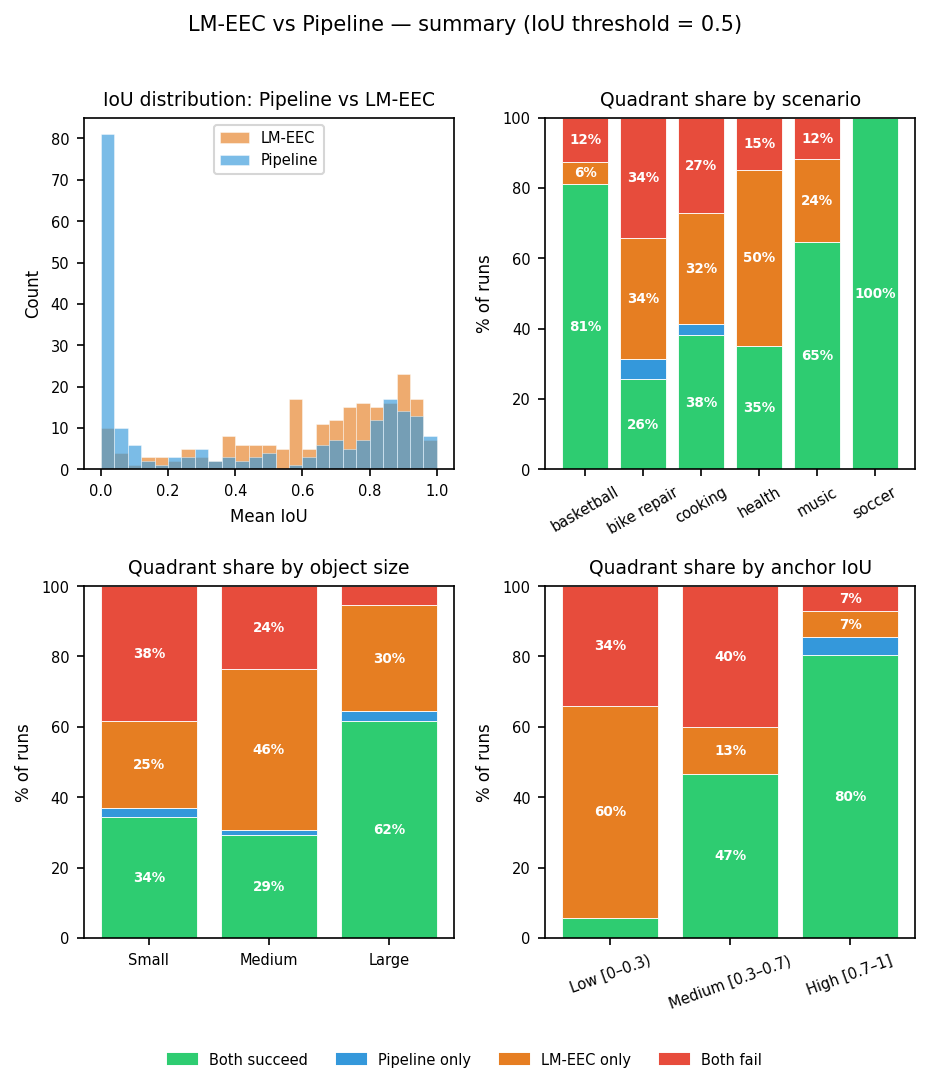
\includegraphics[width=\linewidth]{imgs/ch4/pipeline-lmeec.png}
    \caption{Comparison of the full pipeline against LM-EEC on the \textit{Exo2Ego} validation takes at an IoU threshold of 0.5. The top left panel overlays the two IoU distributions. The remaining panels split every run into one of four outcomes, namely both succeed, pipeline only, LM-EEC only, and both fail, broken down by scenario (top right), object size (bottom left), and anchor IoU (bottom right).}
    \label{fig:pipeline-lmeec}
\end{figure}

The same split recurs whenever we slice the data. By scenario, the strongest regimes are basketball (81\% joint success) and music (65\%), whereas bike repair is the weakest at 26\%, with both methods failing on 34\% of its runs. Bike repair concentrates small objects whose identity is ambiguous to name, which is precisely where the language bridge of Stage~2 struggles to carry the object across views. Object size tells the same story, since joint success holds near 34\% on small and 29\% on medium objects and then jumps to 62\% on large ones, while the rate at which both methods fail drops from 38\% to 5\%. LM-EEC tracks the same pattern, so the difficulty is shared rather than specific to our pipeline. Interestingly, the small and medium regimes are almost identical, which suggests the penalty sets in below a size threshold rather than scaling smoothly with it.

Crucially, the breakdown by anchor IoU locates the failure. When the anchor IoU is high (in $[0.7,1]$), both methods succeed jointly in 80\% of cases and LM-EEC's advantage shrinks to 7\%. When it is low (in $[0,0.3)$), the pipeline collapses to 5\% joint success while LM-EEC alone wins 60\% of those cases. The state of the art therefore dominates exactly where our anchors are poor, which marks anchor selection and object description as the directions with the highest leverage for improvement.

% ------------------------------------------------------------
\section{Mechanistic Analysis of Performance}
\label{sec:gap-analysis}
% ------------------------------------------------------------

In the previous section we identified a concentrated symptom of our pipeline. Because every intermediate output of the pipeline is legible, we can assign each dead case to the stage that lost it. We conduct this analysis on 25\% of the validation split of $\dataset$, comparing against the two strongest runs of the pipeline in each direction, namely 218 triplets $(\take, o, d)$ of a take, an object, and a direction per run across 45 takes and 172 distinct objects. Every number below is computed against the ground truth masks.

\paragraph{The gap is bimodal.}
\label{subsec:bimodal}

Half of the deficit is a discrete failure and half is ordinary imprecision. Splitting the mean IoU into a mass near zero and the rest, the zero mass holds 32\% of cases in \textit{Ego2Exo} and 31\% in \textit{Exo2Ego}, while the mean over the surviving cases climbs to 0.569 and 0.617 (\cref{tab:bimodal}). Removing the zero mass alone would lift the average by roughly 0.18 in both directions, matching the state of the art set by LM-EEC (\cref{tab:main}). Hence the name ``dead'' mass, since the cases in it are not weak predictions but absent ones. We dissect this in the remainder of this section.

\begin{table}
  \centering
  \setlength{\tabcolsep}{6pt}
  \caption{The IoU deficit split into a dead mass and a working mode.}
  \label{tab:bimodal}
  \begin{tabular}{lcc}
  \toprule
  & \textit{Ego2Exo} & \textit{Exo2Ego} \\
  \midrule
  Mean IoU (all cases)        & 0.389 & 0.428 \\
  Dead mass (IoU $<$ 0.01)    & 32\%  & 31\%  \\
  Mean IoU (working mode)     & 0.569 & 0.617 \\
  Lift from removing dead mass & $+0.180$ & $+0.189$ \\
  \bottomrule
  \end{tabular}
\end{table}

\paragraph{The loss is born at the anchor.}
\label{subsec:born-at-anchor}

The dead cases are created when the object is transferred across views, not during temporal propagation. The anchor IoU, measured on the anchor frame itself before any propagation, is exactly zero in 37\% of the subset in both directions, and only about one in ten of those ever recovers to a final IoU above 0.1. Naturally, checking anchor IoU is unfeasible since it requires access to ground truth masks in the destination view. Thus, a dead anchor remains dead. The opposite event, a healthy anchor that collapses during propagation, accounts for only 8\% of the subset in \textit{Ego2Exo} and 6\% in \textit{Exo2Ego}. This isolates Stages~2 and~3, the language bridge and its grounding, as the stage that decides the dead mass, and it further validates the design of \cref{subsec:Stage4}; on a good anchor, it rarely loses the object in subsequent and preceding frames.

Two features of this failure stand out. First, this is a challenging problem because it is a silent failure. A mask is produced in 93\% of the dead cases, so the pipeline almost never abstains. Instead, it commits to a wrong answer. Second, these are not failures of object visibility. Every dead case shows the true object on the destination frame, and none has the object absent from the view entirely. In other words, we are not asking the pipeline something that is not there, but rather the pipeline ``hooks'' on the wrong object, and there is no inherent gate that checks whether the produced mask is on the right object.

Next, we ask what drives a case into that mass and where across those two stages the loss first lands.

\paragraph{Object size and naming are drivers.}
\label{subsec:drivers}

Two factors push a case into the dead mass, and they act independently. The first is object size. In \textit{Ego2Exo} the rate of anchor failure falls monotonically from 63\% on the smallest size quartile to 18\% on the largest, because the destination camera mounted on the head renders objects small and a small object gives both the detector and the segmenter little to lock onto. In \textit{Exo2Ego} the relationship is flat across the lower three quartiles, near 44\%, and improves only at the largest, so the size effect is real but depends on the direction.

The second driver is the object name the VLM writes, and it hurts on top of size rather than through it. Holding size fixed, a name that does not match the ground truth object roughly doubles to triples the rate of anchor failure in every size bucket, and marginally it raises that rate from 24\% to 61\% in \textit{Ego2Exo} and from 16\% to 53\% in \textit{Exo2Ego}. Even on large and clearly visible objects a wrong name fails about half the time. The two directions weight the drivers differently, with the \textit{Ego2Exo} dead mass leaning on size and the \textit{Exo2Ego} dead mass leaning on naming, but the single largest cell in both is the object that is at once small and misnamed. This suggests that SAM 3 agent segmentation is sensitive to subtle shifts in meaning that language can have with synonyms or objects of similar look.

\paragraph{Failure waterfall.}
\label{subsec:waterfall}

Charging each dead case to the first stage that fails turns these drivers into an ordering. We build \cref{tab:waterfall} by walking the pipeline in sequence and stopping at the first stage that breaks. It shows that naming in Stage~2 is the single largest cause by a wide margin, accounting for 59\% of the dead mass in \textit{Ego2Exo} and 81\% in \textit{Exo2Ego}. Selecting the anchor frame in Stage~3 is next, and the two together explain 74\% and 92\% of all dead cases. Grounding DINO placing its box off the object and the agent segmenting the wrong thing inside a good box are real but minor by comparison. Notably, propagation is zero by construction, since an anchor on the wrong object will reliably stay for the entirety of propagation. Therefore, the bulk of the loss is produced before SAM~3 ever runs, pointing to the need for more thorough analysis of VLM descriptions than our approach in \cref{sec:ablations}.

\begin{table}
  \centering
  \setlength{\tabcolsep}{5pt}
  \caption{Failure waterfall over the dead mass per direction, charging each case to the first stage that fails. Cells are shares of the dead mass.}
  \label{tab:waterfall}
  \begin{tabular}{llcc}
  \toprule
  Stage & First failure & \textit{Ego2Exo} & \textit{Exo2Ego} \\
  \midrule
  Stage~2 & VLM names a different object        & 59\% & 81\% \\
  Stage~3 & Anchor frame lands on a tiny object   & 15\% & 11\% \\
  Stage~3 & Grounding DINO box misses the object & 10\% & 2\%  \\
  Stage~3 & Agent segments wrong despite a good box & 16\% & 5\% \\
  Stage~4 & Propagation                          & 0\%  & 0\%  \\
  \midrule
          & Total                                & 100\% & 100\% \\
  \bottomrule
  \end{tabular}
\end{table}

Reading the waterfall back through \cref{chap:theory} clarifies why naming dominates. The language bridge of \cref{subsec:Stage2} asks a general VLM to name a target it sees only as a translucent overlay on a full frame. When that target occupies a fraction of a percent of the image, is ambiguous, or can have multiple names, the model describes the salient object using the features it can extract. The bridge is only as good as the object description it carries over to the other view.

\paragraph{Why the model names the wrong object.}
\label{subsec:Stage2-deepdive}

The naming failure is one of perception, not of vocabulary or implementation. On the dead cases the source mask handed to the model is three to six times smaller than on the successful ones (median 1.43\% against 4.05\% of the frame in \textit{Ego2Exo}, and 0.098\% against 0.564\% in \textit{Exo2Ego}), and in \textit{Exo2Ego} half of the failures show the object at under 0.1\% of the frame. Crucially, when the model misnames it names a different object that is itself annotated in the same take in 38\% of \textit{Ego2Exo} and 24\% of \textit{Exo2Ego} failures, so it describes a real and clearer neighbour rather than hallucinating. The call runs deterministically and without a description cache, which rules out a software cause, and genuine vocabulary near misses such as ``a plate'' read as ``a bowl'' form a small minority. The pattern holds once we look past the separately annotated neighbours. Across all dead cases, the model never hallucinates an absent object but always nominates a real and generally larger structure present alongside the target. \Cref{tab:wrong-nomination} reports the split, where a minority are named correctly and die downstream, while of the genuine naming failures roughly a quarter name a separately annotated neighbour and the remainder name an object present in the scene yet outside the annotation set. Typically, this is the dominant container, tool, or surface on which the tiny target rests, with true synonyms and generic categories of the right object forming a small residual.

\begin{table}
\centering
\caption{What the VLM nominates on the dead cases ($\mathrm{anchor\ IoU}=0$), as a proportion of all such cases per direction.}
\label{tab:wrong-nomination}
\begin{tabular}{lcc}
\toprule
Nominated object & \textit{Ego2Exo} & \textit{Exo2Ego} \\
\midrule
Correct target (failure is downstream) & 41\% & 19\% \\
A different, separately annotated object in the take & 25\% & 23\% \\
A present but unannotated object (container/tool/surface) & 34\% & 58\% \\
\bottomrule
\end{tabular}
\end{table}


\paragraph{Cropping the input is ineffective.}
\label{subsec:crop}

The logical remedy to the above problem is to crop the seed frame to the target object so it becomes the predominant element of the input of the VLM. Strikingly, replacing the full frame with a tight crop of the object lowers IoU from 0.411 to 0.180, more than halving it, and the collapse is consistent case by case (\cref{tab:crop}). The hypothesis is that identity of a small object is carried by its surroundings, so a crop that maximises the object's pixels destroys the very evidence the VLM uses to name it. Looking at some qualitative examples, the VLM reads a cropped basketball as a finger, a CPR manikin as a human hand, and a pack of noodles as pink paper. The one form of cropping that survives is additive, appending a zoom alongside the full frame rather than replacing it, which neither helps nor harms at this threshold. 

\paragraph{Confident mis-groundings.}
\label{subsec:confident-wrong}

Naming in Stage~2 decides most of the dead mass, but the rest is charged to Stage~3, where Grounding DINO and the SAM~3 agent act on a name that is already correct. Grounding DINO reports high confidence on these cases, with a median top score of 0.53 in \textit{Ego2Exo} and 0.73 in \textit{Exo2Ego} and nothing below 0.30, and the SAM~3 agent marks its own output acceptable on the majority of them. Worse, these confidence values overlap almost completely with those of the successful cases, so no internal signal the pipeline already computes can tell a hit from a miss. We call this failure a ``confident mis-grounding'', because the pipeline is not uncertain and recovering, but certain and wrong.

\paragraph{Extending the ill cases.}
\label{subsec:ill-cases}

Restricting the analysis to exact zeros understates the prize and hides a second failure mode. Widening the target to every case below 0.3 IoU, namely ``ill cases'', roughly doubles the affected population, to 51\% of cases in \textit{Ego2Exo} and 49\% in \textit{Exo2Ego}. Additionally, this band carries about 80\% of the total deficit, so almost everything worth fixing sits below 0.3. The band is not simply a softer copy of the zeros. The share of cases with a dead anchor falls from about 95\% at exact zero to roughly 37\% across the band, while propagation drift rises from near zero to about 30\% of the added cases. Extending the target therefore surfaces a Stage~4 problem that the dead mass alone hid completely.

That drift mode has a clean signature of its own. Looking at drifting cases, the segmentation correctly peaks at the anchors and then loses the mask entirely on 65\% to 75\% of the remaining frames. The object is not sliding onto a nearby blob, as it does at a failed anchor, but rather the mask goes empty and stays empty. Long clips drift more in both directions, anchors clustered in one short stretch of a long clip drift more in \textit{Ego2Exo}, and in \textit{Exo2Ego} the small exocentric object simply leaves the frame and the tracker does not re-capture it. Unlike the silent dead mass, this failure announces itself, since a long run of empty masks between ones that are not empty is an internal signal that can be exploited.

\paragraph{What the analysis points to.}
\label{subsec:gap-summary}

Three findings organise everything above. The pipeline's deficit is concentrated in a dead mass of confident mis-groundings. That mass is born at the language bridge rather than in tracking. And within it, the dominant cause is a VLM naming a tiny object after the larger neighbour it can actually see. These point to a corresponding set of directions, namely (i) constraining Stage~2 to a canonical noun phrase while preserving the scene context the name depends on, (ii) an external verification signal that fires on the confident and wrong cases the model's own confidence cannot separate, and (iii) a trigger that reacquires the object on runs of empty masks to recover the propagation drift that only appears once the target widens beyond exact zeros. Each rests on the same property that made this analysis possible, that a pipeline of frozen and legible stages exposes where it breaks. Before turning these directions into future work in \cref{chap:conclusions}, we test in \cref{sec:interventions} whether direct interventions against the naming bottleneck and the confident wrong groundings already close the gap.

% ------------------------------------------------------------
\section{Targeted Interventions}
\label{sec:interventions}
% ------------------------------------------------------------

The legibility that exposed these failures also lets us attack them directly. We report three interventions, each aimed at a stage the analysis charged with the dead mass. Their outcomes are mostly negative, and we include them because a negative result on a legible pipeline still localises the constraint, which sharpens the future work of \cref{chap:conclusions}.

\paragraph{Conditioning the description on scene vocabulary.}
The waterfall placed naming at the head of the dead mass, and the first direction of \cref{subsec:gap-summary} asks for the scene context that a bare object name discards. We add a stage after Block~1 that classifies the take into its scenario, maps that scenario to a curated list of plausible object names, and hands the list to Block~2, so the generated description is anchored to a known vocabulary rather than invented from the overlay alone. The intervention is encouraging on the smaller subset, lifting IoU from 0.376 to 0.408 in \textit{Ego2Exo} and from 0.322 to 0.480 in \textit{Exo2Ego} on 10\% of the validation set, but the gain narrows to $+0.011$ and reverses to $-0.008$ on the 25\% subset (\cref{tab:abl-vlm-align}). The effect does not yet survive the larger sample, so we record scene conditioning as the most direct lever on the naming bottleneck and the clearest candidate for a canonical naming fix, pending evaluation on the full validation set.

\begin{table}[h]
  \centering\small
  \setlength{\tabcolsep}{6pt}
  \caption{Scene vocabulary conditioning of the description, anchors ranked by confidence, on two validation subsets.}
  \label{tab:abl-vlm-align}
  \begin{tabular}{llcc}
  \toprule
  Subset & Conditioning & \textit{Ego2Exo} IoU$\uparrow$ & \textit{Exo2Ego} IoU$\uparrow$ \\
  \midrule
  10\% & Off & 0.376 & 0.322 \\
  10\% & On  & \textbf{0.408} & \textbf{0.480} \\
  \midrule
  25\% & Off & 0.378 & \textbf{0.437} \\
  25\% & On  & \textbf{0.389} & 0.429 \\
  \bottomrule
  \end{tabular}
\end{table}

\paragraph{Cropping the destination detection.}
A second family of dead cases survives correct naming, where Grounding DINO and the agent lock onto a large neighbour of the target. Cropping the source frame for the VLM already proved counterproductive in \cref{subsec:crop}, but that crop starved the description of context. Here we crop on the destination side instead, passing the Grounding DINO box to the SAM~3 agent as a hint and segmenting within it. In aggregate the hint hurts in all four combinations of direction and ranking, by $-0.044$ and $-0.043$ in \textit{Ego2Exo} and $-0.005$ and $-0.043$ in \textit{Exo2Ego}. Stratifying by the baseline IoU of each frame explains the loss (\cref{tab:abl-crop-strat}), since the hint rescues frames the pipeline was already failing, adding 0.043 to 0.077 in the low baseline band, yet corrupts frames the pipeline already handled, removing 0.076 to 0.217 in the high band, and the population the pipeline already handles is large enough to drive the mean negative.

The thin payoff in the failing band is not a fault of the crop but of what precedes it. When the VLM mislabels the object, Grounding DINO confidently boxes the wrong one and the crop faithfully zooms into that wrong object, so the hint cannot recover a case that naming has already lost (\cref{subsec:Stage2-deepdive}). An unconditional hint is therefore the wrong tool, and only a gated variant that fires on the failing population without touching the rest could net positive.

\begin{table}[h]
  \centering\small
  \setlength{\tabcolsep}{5pt}
  \caption{Destination crop hint stratified by the baseline IoU of each frame, 25\% validation. Rank is the anchor ranking rule, by confidence (conf) or box area (area). The hint helps the low baseline band and harms the high band, and the large high band drives the negative mean.}
  \label{tab:abl-crop-strat}
  \begin{tabular}{lllrccc}
  \toprule
  Direction & Rank & Baseline band & $n$ & Off & On & $\Delta$ \\
  \midrule
  \textit{Ego2Exo} & conf & Low $[0,0.25)$   & 17257 & 0.015 & 0.064 & $+0.049$ \\
  \textit{Ego2Exo} & conf & Mid $[0.25,0.6)$ &  2407 & 0.435 & 0.499 & $+0.063$ \\
  \textit{Ego2Exo} & conf & High $[0.6,1]$   & 12432 & 0.870 & 0.676 & $-0.194$ \\
  \cmidrule(l){2-7}
  \textit{Ego2Exo} & area & Low $[0,0.25)$   & 18047 & 0.011 & 0.088 & $+0.077$ \\
  \textit{Ego2Exo} & area & Mid $[0.25,0.6)$ &  2329 & 0.431 & 0.318 & $-0.113$ \\
  \textit{Ego2Exo} & area & High $[0.6,1]$   & 11720 & 0.866 & 0.651 & $-0.215$ \\
  \midrule
  \textit{Exo2Ego} & conf & Low $[0,0.25)$   & 15916 & 0.009 & 0.065 & $+0.056$ \\
  \textit{Exo2Ego} & conf & Mid $[0.25,0.6)$ &  1338 & 0.435 & 0.494 & $+0.059$ \\
  \textit{Exo2Ego} & conf & High $[0.6,1]$   & 14842 & 0.896 & 0.820 & $-0.076$ \\
  \cmidrule(l){2-7}
  \textit{Exo2Ego} & area & Low $[0,0.25)$   & 21353 & 0.007 & 0.051 & $+0.043$ \\
  \textit{Exo2Ego} & area & Mid $[0.25,0.6)$ &   952 & 0.430 & 0.228 & $-0.202$ \\
  \textit{Exo2Ego} & area & High $[0.6,1]$   &  9791 & 0.902 & 0.685 & $-0.217$ \\
  \bottomrule
  \end{tabular}
\end{table}

\paragraph{Brightening the egocentric view.}
Egocentric frames are often dark, which suggested that part of the dead mass might be a problem of raw visibility. Raising the brightness and contrast of the egocentric frames before description and segmentation does not help, and instead lowers IoU by 0.037 in \textit{Ego2Exo} and 0.023 in \textit{Exo2Ego}, within the range of variation between runs (\cref{tab:abl-bright}). Visibility at the pixel level is therefore not the binding constraint, which is consistent with the earlier finding that the dead cases show the object plainly and fail at naming rather than at the perception of light (\cref{subsec:born-at-anchor}).

\begin{table}[h]
  \centering\small
  \setlength{\tabcolsep}{6pt}
  \caption{Brightness and contrast augmentation of the egocentric frames, 25\% validation, anchors ranked by confidence.}
  \label{tab:abl-bright}
  \begin{tabular}{lccc}
  \toprule
  Direction & Off & On & $\Delta$ \\
  \midrule
  \textit{Ego2Exo} & 0.378 & 0.341 & $-0.037$ \\
  \textit{Exo2Ego} & 0.437 & 0.414 & $-0.023$ \\
  \bottomrule
  \end{tabular}
\end{table}

Each of these interventions localises the constraint without lifting it. We carry the resulting directions, together with the need for a more discriminative grounding detector on the remaining slice of the waterfall where Grounding DINO boxes a correctly named object off target, into \cref{chap:conclusions}.